\documentclass[border=2pt]{standalone}
\usepackage{amssymb,amsmath}
\usepackage{tikz-cd}
\usepackage{physics}
\usetikzlibrary{arrows}

\usepackage{tikz}
\let\OX\bigotimes
\newcommand{\OP}{\displaystyle\bigoplus}
\let\ox\otimes
\let\op\oplus
\let\isom\cong
\let\vf\varphi
\begin{document}


\tikzset{every picture/.style={line width=0.75pt}} %set default line width to 0.75pt        

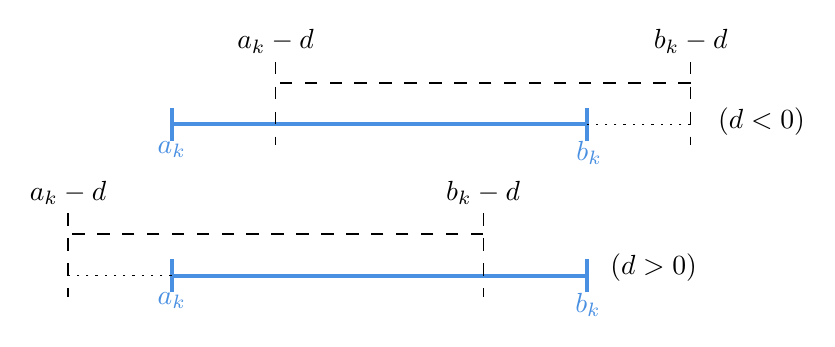
\begin{tikzpicture}[x=0.75pt,y=0.75pt,yscale=-1,xscale=1]
%uncomment if require: \path (0,300); %set diagram left start at 0, and has height of 300

%Straight Lines [id:da9341655393999668] 
\draw [color={rgb, 255:red, 74; green, 144; blue, 226 }  ,draw opacity=1 ][line width=1.5]    (372,113) -- (172,113) ;
\draw [shift={(172,113)}, rotate = 360] [color={rgb, 255:red, 74; green, 144; blue, 226 }  ,draw opacity=1 ][line width=1.5]    (0,8.05) -- (0,-8.05)   ;
\draw [shift={(372,113)}, rotate = 360] [color={rgb, 255:red, 74; green, 144; blue, 226 }  ,draw opacity=1 ][line width=1.5]    (0,8.05) -- (0,-8.05)   ;
%Straight Lines [id:da6039036674811626] 
\draw  [dash pattern={on 4.5pt off 4.5pt}]  (222,83) -- (222,123) ;
%Straight Lines [id:da1513548346981024] 
\draw [color={rgb, 255:red, 0; green, 0; blue, 0 }  ,draw opacity=1 ][line width=0.75]  [dash pattern={on 4.5pt off 4.5pt}]  (422,93) -- (222,93) ;
%Straight Lines [id:da16722830339355022] 
\draw  [dash pattern={on 0.84pt off 2.51pt}]  (422,113) -- (372,113) ;
%Straight Lines [id:da18428775516405282] 
\draw  [dash pattern={on 4.5pt off 4.5pt}]  (422,83) -- (422,123) ;
%Straight Lines [id:da09837624298314163] 
\draw [color={rgb, 255:red, 74; green, 144; blue, 226 }  ,draw opacity=1 ][line width=1.5]    (372,186) -- (172,186) ;
\draw [shift={(172,186)}, rotate = 360] [color={rgb, 255:red, 74; green, 144; blue, 226 }  ,draw opacity=1 ][line width=1.5]    (0,8.05) -- (0,-8.05)   ;
\draw [shift={(372,186)}, rotate = 360] [color={rgb, 255:red, 74; green, 144; blue, 226 }  ,draw opacity=1 ][line width=1.5]    (0,8.05) -- (0,-8.05)   ;
%Straight Lines [id:da6556590238526158] 
\draw  [dash pattern={on 4.5pt off 4.5pt}]  (122,156) -- (122,196) ;
%Straight Lines [id:da31526877430040756] 
\draw [color={rgb, 255:red, 0; green, 0; blue, 0 }  ,draw opacity=1 ][line width=0.75]  [dash pattern={on 4.5pt off 4.5pt}]  (322,166) -- (122,166) ;
%Straight Lines [id:da32523039485023275] 
\draw  [dash pattern={on 0.84pt off 2.51pt}]  (172,186) -- (122,186) ;
%Straight Lines [id:da8025330005794951] 
\draw  [dash pattern={on 4.5pt off 4.5pt}]  (322,156) -- (322,196) ;

% Text Node
\draw (172,193) node [anchor=north] [inner sep=0.75pt]  [color={rgb, 255:red, 74; green, 144; blue, 226 }  ,opacity=1 ]  {$a_{k}$};
% Text Node
\draw (380,193) node [anchor=north east] [inner sep=0.75pt]  [color={rgb, 255:red, 74; green, 144; blue, 226 }  ,opacity=1 ]  {$b_{k}$};
% Text Node
\draw (122,153) node [anchor=south] [inner sep=0.75pt]  [color={rgb, 255:red, 0; green, 0; blue, 0 }  ,opacity=1 ]  {$a_{k} -d$};
% Text Node
\draw (322,153) node [anchor=south] [inner sep=0.75pt]  [color={rgb, 255:red, 0; green, 0; blue, 0 }  ,opacity=1 ]  {$b_{k} -d$};
% Text Node
\draw (172,120) node [anchor=north] [inner sep=0.75pt]  [color={rgb, 255:red, 74; green, 144; blue, 226 }  ,opacity=1 ]  {$a_{k}$};
% Text Node
\draw (380.52,120) node [anchor=north east] [inner sep=0.75pt]  [color={rgb, 255:red, 74; green, 144; blue, 226 }  ,opacity=1 ]  {$b_{k}$};
% Text Node
\draw (222,80) node [anchor=south] [inner sep=0.75pt]  [color={rgb, 255:red, 0; green, 0; blue, 0 }  ,opacity=1 ]  {$a_{k} -d$};
% Text Node
\draw (422,80) node [anchor=south] [inner sep=0.75pt]  [color={rgb, 255:red, 0; green, 0; blue, 0 }  ,opacity=1 ]  {$b_{k} -d$};
% Text Node
\draw (382,174) node [anchor=north west][inner sep=0.75pt]    {$( d >0)$};
% Text Node
\draw (434,104) node [anchor=north west][inner sep=0.75pt]    {$( d< 0)$};


\end{tikzpicture}


\end{document}